% !TEX encoding = UTF-8 Unicode

\documentclass[9pt, openany]{extbook}
\usepackage{Genesys}
\usepackage{hyperref}
\geometry{papersize={5.5in, 8.5in}}
\usepackage{wrapfig}
\graphicspath{{img/}}
\newfontfamily\TF{Gemina 2 Regular}
\setcounter{tocdepth}{1}


\usepackage{eso-pic}

\newcommand\BackgroundPic{%
\hspace*{-0.2\paperwidth}
\parbox[b][\paperheight]{\paperwidth}{%
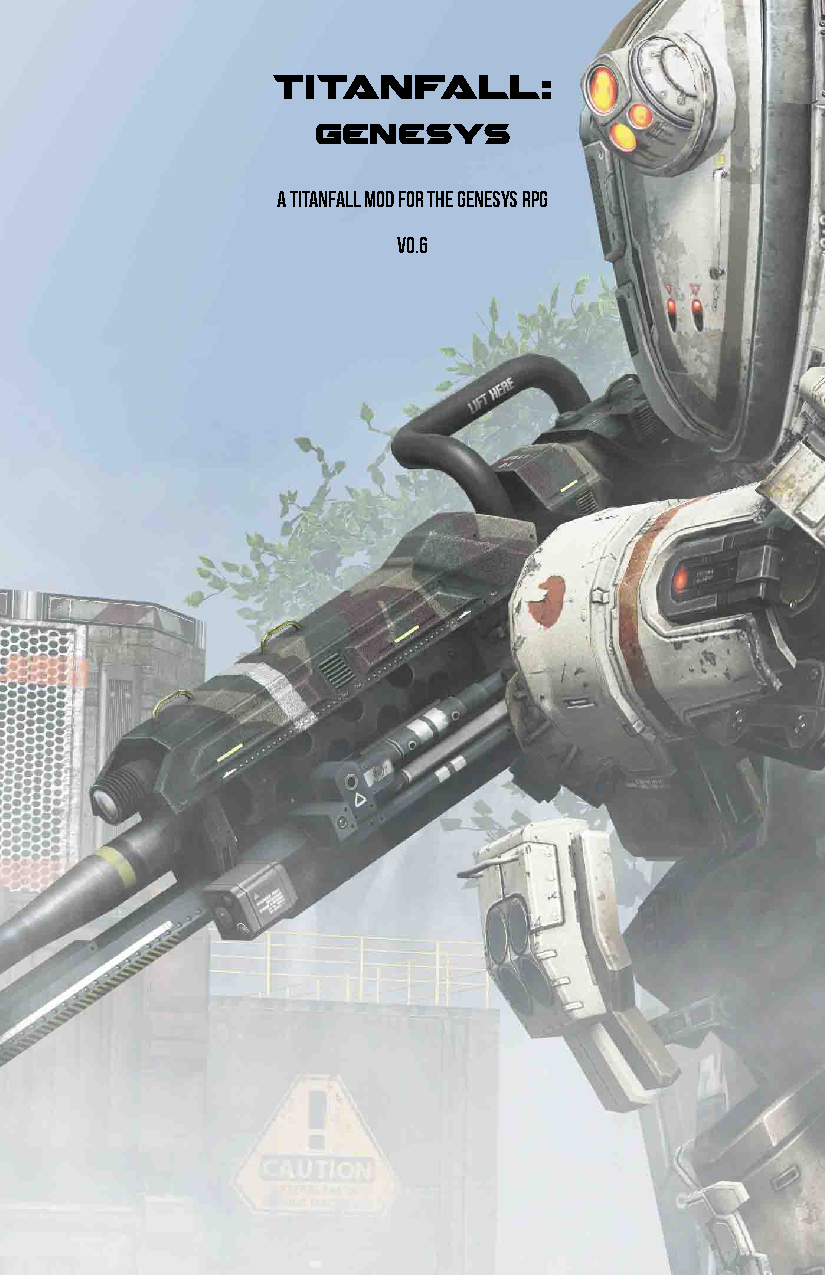
\includegraphics[keepaspectratio, height=\paperheight]{Titanfall.jpg}%
}}




\begin{document}
\AddToShipoutPicture*{\BackgroundPic}

\thispagestyle{empty}
%\vspace*{2em}
{\noindent\centering\Huge\TF titanfall:\\{\huge Genesys}\\[1em]{\Large\sffamily\bfseries A Titanfall Mod for the Genesys RPG\\v0.5}\\}
\vspace*{\fill}

\clearpage
\pagenumbering{roman}
\begin{multicols}{2}
\tableofcontents
\end{multicols}



\clearpage
\pagenumbering{arabic}
\setcounter{page}{1}



%%%%%
% Titans
%%%%%

\chapter{Titans}
\label{chap:titans}

Titans are mech-style robots, descended from modern-day fledgling military exoskeletons, designed for both civilian and military applications. 

There are three classes of titans, as described below.

\section{Special Rules}
\label{sec:specialrules}

All titans have the following special rule:

\textbf{Mecha Chassis:} As long as a Titan's propulsion isn't compromised it ignores the speed requirement for the reposition maneuver.

\section{Stryder}
\label{sec:stryder}
\begin{wrapfigure}[13]{r}{.34\linewidth}
\vspace*{-2em}
\includegraphics[width=\linewidth]{Stryder}
\end{wrapfigure}


The Stryder is a Titan chassis developed and manufactured by Hammond Robotics. Developed as an extremely mobile and maneuverable Titan variant, the Stryder's almost skeletal design has been optimized for superior speed and agility. Significant improvements have been made to its Dash Core, while the Titan can also sprint for greater distances, making it perfect for hit-and-run attacks, ambushes and rapid redeployments. Unfortunately, this speed comes at a price. The Stryder's design is stripped down compared to other Titan variants, and its armor is largely non-existent, making it much more fragile in combat. In Titan-vs-Titan engagements, Stryder Pilots must use all available cover and their machine's impressive speed to outflank and evade their heavier adversaries, as they are unlikely to survive a straight-up slug-fest.

\textbf{Dash Core}: The Stryder-class Titan has an in-built dash core. Once per round on your turn, you may cause the titan to suffer 1 system strain to perform the Evade maneuver as an Incidental, ignoring the Speed requirement.

\vspace{2em}

\Vehicle{3}{3}{+2}{2}{1}{13}{20}

\begin{multicols}{2}
\noindent\textbf{Control Skill:} Pilot (Titan)\\
\noindent\textbf{Complement:} One pilot\\
\noindent\textbf{Passenger Capacity:} None\\
\noindent\textbf{Price/Rarity:} 20,750/8\\
\noindent\textbf{Consumables:} None\\
\noindent\textbf{Encumbrance Capacity:} 2\\
\noindent\textbf{Weapons:} Titan punch (Pilot [Titan]; Damage 2; Critical 3; Range [Engaged]; Accurate 1)\\
\noindent\textbf{Hard Points:} 3
\end{multicols}

\section{Atlas}
\label{sec:atlas}
\begin{wrapfigure}{l}{.34\linewidth}
\includegraphics[width=\linewidth]{Atlas}
\end{wrapfigure}


The Atlas is the original Titan model produced by Hammond Robotics. It has a balance of mobility and armor, having more mobility than the Ogre, but more armor than the Stryder. This was the first Titan to be revealed.

The Atlas seems to be the second tallest Titan model, though exact measurements are unknown. Based on photos of the Atlas standing next to a pilot, it can be estimated to be between 20-25 feet tall. Its main entry point is in its chest, which opens up for the player. The Atlas also has a secondary entry point---a small hatch in the top. This is also the eject port for the Atlas.

The Atlas is the oldest Titan model on the Frontier and has instigated the development of both the Stryder and Ogre patterns. It was used through the Titan Wars, and onto the Frontier War. The Atlas is equipped with a Damage Core, which, when ready, the pilot can activate on command to substantially increase damage dealt by the titan.

\textbf{Damage Core}: The Atlas-class Titan has an in-built damage core. Once per round on your turn, you may cause the titan to suffer 1 system strain to perform the Aim maneuver as an Incidental.\\[1em]

\Vehicle{3}{2}{+0}{2}{2}{15}{15}

\begin{multicols}{2}
\noindent\textbf{Control Skill:} Pilot (Titan)\\
\noindent\textbf{Complement:} One pilot\\
\noindent\textbf{Passenger Capacity:} None\\
\noindent\textbf{Price/Rarity:} 21,750/8\\
\noindent\textbf{Consumables:} None\\
\noindent\textbf{Encumbrance Capacity:} 2\\
\noindent\textbf{Weapons:} Titan punch (Pilot [Titan]; Damage 2; Critical 3; Range [Engaged])\\
\noindent\textbf{Hard Points:} 3
\end{multicols}

\vspace*{\fill}
\pagebreak

\section{Ogre}
\label{sec:ogre}
\begin{wrapfigure}[12]{r}{.34\linewidth}
\vspace*{-2em}
\includegraphics[width=\linewidth]{Ogre}
\end{wrapfigure}

The H-KA02/a Ogre Heavy Titan is a Titan model produced by Hammond Armament Division and Wonyeon Defense. Developed as an extremely tough Titan chassis, the Ogre's design has been compared to a main battle tank, optimized for taking higher amounts of damage and dealing out more than the Atlas or Stryder Titans. The Ogre stands slightly taller than the Atlas and has bulkier armor. The main entry point of an Ogre is via a large hatch on its top rather than the chest, like the Atlas or Stryder. The Ogre is equipped with a Shield Core, which amps the Titan's shield for a limited time.

\textbf{Shield Core}: The Ogre-class Titan has an in-built shield core. Once per round on your turn, you may cause the titan to suffer 1 system strain to perform the Brace for Impact maneuver as an Incidental.\\[3em]

\Vehicle{3}{1}{-2}{2}{2}{18}{18}


\begin{multicols}{2}
\noindent\textbf{Control Skill:} Pilot (Titan)\\
\noindent\textbf{Complement:} One pilot\\
\noindent\textbf{Passenger Capacity:} None\\
\noindent\textbf{Price/Rarity:} 25,740/8\\
\noindent\textbf{Consumables:} None\\
\noindent\textbf{Encumbrance Capacity:} 2\\
\noindent\textbf{Weapons:} Titan punch (Pilot [Titan]; Damage 2; Critical 3; Range [Engaged]; Vicious 1)\\
\noindent\textbf{Hard Points:} 3
\end{multicols}



No Titan is complete without its weapons. Most Titans have one primary, handheld weapon, one ordnance launcher and one defensive system. Some pilots prefer to change it up a bit and go for extra defense or offense. 

\section{Titan Weapons}

Each main weapon takes up one hard point on the Titan.

\subsection{40mm Cannon}

\begin{wrapfigure}[3]{l}{.34\linewidth}
\vspace*{-2em}
\includegraphics[width=\linewidth]{40mmCannon}
\end{wrapfigure}

The factory issue 40mm Cannon is a semi-automatic weapon that fires a high-explosive round with good accuracy. 

\subsection{Arc Cannon}
\begin{wrapfigure}[4]{r}{.34\linewidth}
\vspace*{-2em}
\includegraphics[width=\linewidth]{ArcCannon}
\end{wrapfigure}

The factory issue Arc Cannon fires a bolt of lightning that propagates across multiple targets. It can be fired quickly, or charged up over time for an increase in firepower. If you perform the Prepare maneuver, increase the damage of one hit of the next combat check by 1 and an arc cannon can negate Defense granted by energy shields by spending \Advantage\Advantage.

\subsection{PR-01 Plasma Railgun}
\begin{wrapfigure}[3]{l}{.34\linewidth}
\vspace*{-2em}
\includegraphics[width=\linewidth]{PlasmaRailgun}
\end{wrapfigure}

The Plasma Railgun is a Titan-sized sniper weapon, used for suppression of armored targets from a distance. The weapon fires a bolt of plasma, accelerated by a system of charged rails.


\subsection{Quad Rocket}
\begin{wrapfigure}[2]{r}{.34\linewidth}
\vspace*{-2em}
\includegraphics[width=\linewidth]{QuadRocket}
\end{wrapfigure}

The Quad Rocket is a weapon that fires a tight-knit cluster of 4 rockets at the target, exploding upon impact.

\subsection{Triple Threat}
\begin{wrapfigure}[4]{l}{.34\linewidth}
\vspace*{-2em}
\includegraphics[width=\linewidth]{TripleThreat}
\end{wrapfigure}

The Triple Threat is a grenade launcher that shoots 3 grenades at once. It excels at clearing rooms, and its grenades explode on armored contact, making it effective at close range against other Titans. Due to the low magazine capacity, however, this weapon can run out of ammo by spending \Threat\Threat\Threat\ (instead of the normal \Despair).

\subsection{XOTBR-16 Chaingun}
\begin{wrapfigure}[3]{r}{.34\linewidth}
\vspace*{-2em}
\includegraphics[width=\linewidth]{XO16Chaingun}
\end{wrapfigure}

The XO-16 Chaingun is a fully automatic ballistic weapon that fires 1.6 inch slugs with high precision at considerable range.

\begin{table}[h!]
\caption{Titan Weapons}
\footnotesize
\begin{GenesysTable}{*{2}{l} *{2}{c} l c r c X[l]}
Name & Skill & Dam & Crit & Range  & HP & Price & Rarity & Special\\
40mm Cannon & Gunnery & 6 & 3 & Long & 1 & 7,750 & 6 & Blast 1, Breach 1 \\
Arc Cannon & Gunnery & 4 & 4 & Medium & 1 & 5,250 & 7 & Blast 3, Special\\
Plasma Railgun & Gunnery & 7 & 2 & Extreme & 1 & 10,750 & 7 & \Special{Accurate 1, Breach 1, Limited Ammo 2}
Quad Rocket & Gunnery & 4 & 3 & Long & 1 & 7,500 & 6 & \Special{Accurate 1, Blast 3, Vicious 2}
Triple Threat & Gunnery & 4 & 4 & Medium & 1 & 8,250 & 7 & \Special{Blast 2, Linked 2, Special}
XO-16 Chaingun & Gunnery & 3 & 4 & Long & 1 & 4,750 & 7 & Auto-fire
\end{GenesysTable}
\end{table}

\section{Titan Ordnance}
Unless otherwise noted, extra reloads for ordnance weapons cost 2,000 credits.

\subsection{Cluster Missile}
\begin{wrapfigure}[4]{l}{.34\linewidth}
\vspace*{-2em}
\includegraphics[width=\linewidth]{ClusterMissile}
\end{wrapfigure}

The Cluster Missile pod fires a missile which, on impact, deploys a shower of secondary explosive charges that continue to explode and saturate an area for a considerable time.

\subsection{Multi-Target Missile System}
\begin{wrapfigure}[3]{r}{.34\linewidth}
\vspace*{-2em}
\includegraphics[width=\linewidth]{MultiTargetMissileSystem}
\end{wrapfigure}

The Multi-Target Missile System enables you to engage multiple targets at once. The Guided quality can only be activated when attacking targets made of significant metal content, like Titans and Spectres.

\subsection{Rocket Salvo}
\begin{wrapfigure}[2]{l}{.34\linewidth}
\vspace*{-2em}
\includegraphics[width=\linewidth]{RocketSalvo}
\end{wrapfigure}

The Rocket Salvo launches a rapid salvo of unguided rockets. Each \Success\  deals +2 damage, instead of +1.

\subsection{Slaved Warheads}
\begin{wrapfigure}[3]{r}{.34\linewidth}
\vspace*{-2em}
\includegraphics[width=\linewidth]{SlavedWarheads}
\end{wrapfigure}

This Titan ordnance pod requires a lock-on before you can fire. When you fire, a barrage of 3 homing missiles will launch towards your locked target. The Guided quality can only be activated when attacking targets made of significant metal content, like Titans and Spectres.


\begin{table}[h!]
\caption{Titan Ordnance}
\footnotesize
\begin{GenesysTable}{*{2}{l} *{2}{c} l c r c X[l]}
Name & Skill & Dam & Crit & Range  & HP & Price & Rarity & Special\\
Cluster Missile & Gunnery & 4 & 3 & Extreme & 1 & 6,250 & 8 & \Special{Blast 4, Breach 1, Limited Ammo 3}
MTM System & Gunnery & 5 & 3 & Extreme & 1 & 9,000 & 8 & \Special{Accurate 1, Auto-Fire, Breach 1, Guided 3, Limited Ammo 3, Special}
Rocket Salvo & Gunnery & 3 & 2 & Long & 1 & 7,050 & 8 & \Special{Blast 1, Breach 2, Inaccurate 1, Limited Ammo 2, Special}
Slave Warhead & Gunnery & 5 & 4 & Long & 1 & 8,250 & 8 & \Special{Blast 1, Breach 1, Guided 2, Limited Ammo 3, Linked 2}
\end{GenesysTable}
\end{table}


%%%%%
% Equipment
%%%%%


\chapter{Equipment}
\label{chap:equip}


\section{Sidearms}
\label{sec:sidearms}

\subsection{b3 Wingman}

\begin{wrapfigure}[4]{l}{.34\linewidth}
\vspace*{-2em}
\includegraphics[width=\linewidth]{B3wingman}
\end{wrapfigure}

The B3 Wingman is an extremely powerful revolver with very high accuracy out to long ranges. Precision aim is required to mitigate the disadvantages of its very low rate of fire. 

\subsection{Hammond P2011}

\begin{wrapfigure}[4]{r}{.34\linewidth}
\vspace*{-2em}
\includegraphics[width=\linewidth]{HammondP2011}
\end{wrapfigure}

The Hammond P2011 is a semi-automatic handgun with good accuracy and damage at range. Its integrated 'match trigger' allows it to be fired very rapidly, which is useful in close quarters. 

\subsection{RE45 Autopistol}

\begin{wrapfigure}[3]{l}{.34\linewidth}
\vspace*{-2em}
\includegraphics[width=\linewidth]{RE45Autopistol}
\end{wrapfigure}


The RE-45 is a fully automatic .45 caliber pistol, sacrificing damage and accuracy at longer distances for improved effectiveness at close range.

\subsection{Smart Pistol mkv}

\begin{wrapfigure}[7]{r}{.34\linewidth}
\vspace*{-2em}
\includegraphics[width=\linewidth]{SmartPistolMK5}
\end{wrapfigure}

The Smart Pistol scans for hostile targets within a short range, locking onto them automatically. Any rounds fired will then maneuver to hit the locked targets. Aiming with the iron sights allows the operator to use the pistol in manual targeting mode. Due to the low magazine capacity, however, this weapon can run out of ammo by spending \Threat\Threat\Threat\ (instead of the normal \Despair). Spare ammunition for the smart pistol is twice the price as normal ammo, 50 credits.

\begin{table}[h!]
\caption{Sidearms}
\footnotesize
\begin{GenesysTable}{*{2}{l} *{2}{c} l c c r c X[l]}
Name & Skill & Dam & Crit & Range & Enc & HP & Price & Rarity & Special\\
B3 Wingman & Ranged (Light) & 6 & 3 & Medium & 1 & 1 & 500 & 3 & \\
Hammond P2011 & Ranged (Light) & 5 & 4 & Medium & 1 & 1 & 150 & 3 & \\
RE-45 Autopistol & Ranged (Light) & 5 & 3 & Short & 2 & 1& 300 & 6 & Accurate 1 \\
Smart pistol mk5 & Ranged (Light) & 5 &  3 & Short & 1 & 1 & 450 & 8 & Guided 3, Special\\

\end{GenesysTable}
\end{table}


\pagebreak
\section{Longarms}
\label{sec:rifles}

\subsection{R101C Carbine}
\begin{wrapfigure}[2]{l}{.34\linewidth}
\vspace*{-2em}
\includegraphics[width=\linewidth]{R101CCarbine}
\end{wrapfigure}


The R-101C is a fully automatic, compact assault weapon commonly used throughout the Frontier. 


\subsection{Hemlock BF-R}
\begin{wrapfigure}[5]{r}{.36\linewidth}
\vspace*{-2em}
\includegraphics[width=\linewidth]{HemlokBFR}
\end{wrapfigure}
The factory issue Hemlok fires a three-round burst. While this can be a liability at short range, this tradeoff allowed the engineers at TW Ordnance to deliver a weapon with a good balance of long-range accuracy, damage, and fire rate.

\subsection{G2A4 Battle Rifle}
\begin{wrapfigure}[4]{l}{.36\linewidth}
\vspace*{-2em}
\includegraphics[width=\linewidth]{G2A4Rifle}
\end{wrapfigure}


Despite recent advances in weapons technology, the older G2A4 semi-automatic rifle remains a favorite of special forces units due to its high damage and extremely precise fire---a testament to its high level of craftsmanship.

\subsection{EVA-8 Shotgun}
\begin{wrapfigure}[5]{r}{.36\linewidth}
\vspace*{-2em}
\includegraphics[width=\linewidth]{EVA8Shotgun}
\end{wrapfigure}


The EVA-8 is a semi-automatic shotgun, originally designed for extra-vehicular activity, both in conventional and in exo-atmospheric conditions. The low capacity and quick trigger means that the EVA-8 can run out of ammo by spending \Threat\Threat\Threat\ (instead of the normal \Despair).

\subsection{R-97 Compact SMG}
\begin{wrapfigure}[3]{l}{.36\linewidth}
\vspace*{-2em}
\includegraphics[width=\linewidth]{R97CompactSMG}
\end{wrapfigure}

The R-97 is a compact submachine gun that excels at close-quarters combat, due to its extremely high rate of fire and minimal recoil.

\subsection{C.A.R. SMG}
\begin{wrapfigure}[4]{r}{.36\linewidth}
\vspace*{-2em}
\includegraphics[width=\linewidth]{CARSMG}
\end{wrapfigure}

The C.A.R. (Combat Advanced Round) submachine gun is designed to fire a more powerful round that provides greater damage and accuracy at range, at the cost of fire rate and capacity.


\subsection{D-101 Longbow DMR}
\begin{wrapfigure}[3]{l}{.36\linewidth}
\vspace*{-2em}
\includegraphics[width=\linewidth]{LongbowDMRSniper}
\end{wrapfigure}

The Longbow-DMR is a semi-automatic sniper rifle. Its hyper-velocity round completely eliminates the need to lead targets, and allows the shooter to fire multiple shots quickly in succession.


\subsection{Kraber-AP Sniper}
\begin{wrapfigure}[4]{r}{.36\linewidth}
\vspace*{-2em}
\includegraphics[width=\linewidth]{KraberAPSniper}
\end{wrapfigure}

The Kraber fires a unique round that ensures 'one-shot, one-kill' results against human-scale targets. However, considerable judgement in leading is required, making this a difficult weapon to use against moving targets.

\subsection{Spitfire LMG}
\begin{wrapfigure}[4]{l}{.36\linewidth}
\vspace*{-2em}
\includegraphics[width=\linewidth]{SpitfireLMG}
\end{wrapfigure}

The Spitfire Light Machine Gun recoils heavily when first fired, but quickly settles into a tight firing pattern. The manufacturer strongly recommends sustained saturating fire, instead of short controlled bursts.



\begin{table}[h!]
\caption{Longarms}
\footnotesize
\begin{GenesysTable}{*{2}{l} *{2}{c} l c c r c X[l]}
Name & Skill & Dam & Crit & Range & Enc & HP & Price & Rarity & Special\\
R101C Carbine & Ranged (Heavy) & 8 & 3 & Long & 4 & 2 & 1,050 & 7 & Auto-fire\\
Hemlock BF-R & Ranged (Heavy) & 8 & 3 & Long & 4 & 2 & 1,000 & 7 & Accurate 1\\
G2A4 Battle Rifle & Ranged (Heavy) & 8 & 3 & Long & 4 & 2 & 950 & 6 &  \\ 
EV-8 Shotgun & Ranged (Heavy) & 8 & 3 & Short & 3 & 2 & 1,250 & 4 & \Special{Blast 6, Knockdown, Special}
R-97 SMG & Ranged (Heavy) & 6 & 3 & Medium & 3 & 2 & 750 & 6 & \Special{Auto-fire, Accurate 1}
C.A.R. SMG & Ranged (Heavy) & 7 & 3 & Medium & 3 & 2 & 550 & 6 & \Special{Accurate 2, Limited Ammo 2}
Longbow DMR & Ranged (Heavy) & 9 & 3 & Long & 4 & 2 & 1,000 & 5 & \Special{Accurate 1, Limited Ammo 3}
Kraber & Ranged (Heavy) & 12 & 2 & Extreme & 5 & 3 & 2,000 & 8 & \Special{Accurate 2, Pierce 2}
Spitfire LMG & Gunnery &10 & 3 & Long & 6 & 3 & 1,750 & 6 & \Special{Auto-fire, Cumbersome 2, Pierce 2, Vicious 2}
\end{GenesysTable}
\end{table}

\section{Pilot Ordnance}
\label{sec:pilotordnance}

\subsection{Special Rules}
\textbf{Set Explosives.} The arc mine is an unusual ordnance in that you don't throw it at your opponent but rather set it in place and wait for someone to trigger the explosion. As an action you may set up to two mines within Engaged range of you. Then, when someone or something enters engaged range with the mine you make an Engineering combat check against the target.


\subsection{Arc Grenade}
\begin{wrapfigure}[4]{r}{.36\linewidth}
\vspace*{-2em}
\includegraphics[width=\linewidth]{ArcGrenade}
\end{wrapfigure}

The Arc Grenade is by infantry of the IMC and Militia. When activated, the Arc Grenade explodes in a blast of Arc energy capable of short circuiting and dealing heavy damage to robotic units and equipment such as Titans, Spectres, Stalkers, HUDs and optical equipment found within the helmet of a Pilot and Reapers. An arc grenade can negate Defense granted by energy shields by spending \Advantage\Advantage.

\subsection{Arc Mine}
\begin{wrapfigure}[6]{l}{.36\linewidth}
\vspace*{-2em}\centering
\includegraphics[width=0.5\linewidth]{ArcMine}
\end{wrapfigure}

The Arc Mine is a proximity mine that can stick on any surface. It takes 1 second after sticking to something to arm. Arc Mines won't explode until an enemy Pilot, Titan, Grunt, or Spectre enter the mine's range. An arc mine can negate Defense granted by energy shields by spending \Advantage\Advantage.


\subsection{Frag Grenade}
\begin{wrapfigure}[2]{r}{.36\linewidth}
\vspace*{-2em}
\includegraphics[width=\linewidth]{FragGrenade}
\end{wrapfigure}

The basic explosive device known to all modern soldiers, the Frag Grenade is still an incredibly useful weapon.

\subsection{Satchel Charge}
\begin{wrapfigure}[6]{l}{.36\linewidth}
\vspace*{-2em}
\centering
\includegraphics[width=.4\linewidth]{SatchelCharge}
\end{wrapfigure}

Satchel Charges stick to any surface and are manually detonated, causing massive explosive damage to anything nearby. Like mines, satchel charges are set and triggered to explode. Unlike a mine, however, you must trigger them yourself. As an action you may place up to two charges within Engaged range. As an out-of-turn incidental you may detonate the charges, making an Engineering combat check against the target.


\begin{table}[h!]
\caption{Ordnance}
\footnotesize
\begin{GenesysTable}{*{2}{l} *{2}{c} l c c r c X[l]}
Name & Skill & Dam & Crit & Range & Enc & HP & Price & Rarity & Special\\
Arc Grenade & Ranged (Light) & 5 & 4 & Short & 1 & 0 & 250 & 6 & \Special{Blast 4, Disorient 2, Limited Ammo 1, Stun Damage, Special}
Arc Mine & Mechanics & 6 & 4 & Engaged & 3 & 0 & 500 & 7 & \Special{Blast 5, Disorient 2, Limited Ammo 1, Stun Damage, Special}
Frag Grenade & Ranged (Light) & 8 & 3 & Short & 1 & 0 & 650 & 7 & \Special{Blast 5, Limited Ammo 1}
Satchel Charge & Mechanics & 12 & 2 & Engaged & 2 & 0 & 2,700 & 6 & \Special{Blast 8, Breach 1, Special}


\end{GenesysTable}
\end{table}



\section{Anti-Titan Weapons}
\label{sec:antititanweapons}


\subsection{Archer Heavy Rocket}
\begin{wrapfigure}[4]{r}{.36\linewidth}
\vspace*{-2em}
\includegraphics[width=\linewidth]{ArcherHeavyRocket}
\end{wrapfigure}

The Archer fires a powerful homing rocket. It must be locked onto a target before it can be fired. When aimed, a targeting window flips out, allowing target acquisition. Hold this window over the target continuously until a lock is achieved, then fire. The Guided quality can only be activated when attacking targets made of significant metal content, like Titans and Spectres. Reload rockets for the Archer cost 3,000 credit.

\subsection{Charge Rifle}
\begin{wrapfigure}[4]{l}{.36\linewidth}
\vspace*{-2em}
\includegraphics[width=\linewidth]{ChargeRifle}
\end{wrapfigure}

The Charge Rifle fires an energy beam that inflicts massive damage. Holding the trigger charges the weapon. Timing is critical to its use: this weapon will only fire when it reaches full charge, and it will discharge automatically as soon as it hits full charge.



\subsection{Mag Launcher}
\begin{wrapfigure}[3]{r}{.36\linewidth}
\vspace*{-2em}
\includegraphics[width=\linewidth]{MagLauncher}
\end{wrapfigure}


The Mag Launcher fires magnetic grenades. When fired, the grenades will veer towards nearby enemy Titans and Spectres, and detonate on impact. The Guided quality can only be activated when attacking targets made of significant metal content, like Titans and Spectres. Due to the low magazine capacity, however, this weapon can run out of ammo by spending \Threat\Threat\Threat\ (instead of the normal \Despair).

\subsection{Sidewinder}
\begin{wrapfigure}[5]{l}{.36\linewidth}
\vspace*{-2em}
\includegraphics[width=\linewidth]{Sidewinder}
\end{wrapfigure}

The Sidewinder is a rapid-fire micro-missile launcher. It is effective against large targets, but lacks precision due to its large spread. The micro-missiles it fires do not yield a large area effect on detonation, due to their shaped-charge design.






\begin{table}[h!]
\caption{Anti-Titan Weapons}
\footnotesize
\begin{GenesysTable}{*{2}{l} *{2}{c} l c c r c X[l]}
Name & Skill & Dam & Crit & Range & Enc & HP & Price & Rarity & Special\\
Archer Rocket & Gunnery & 30 & 2 & Extreme & 8 & 4 & 10,525 & 8 & \Special{Blast 20, Breach 2, Cumbersome 3, Guided 3, Limited Ammo 1, Prepare 1}
Charge Rifle & Gunnery & 9 & 2 & Extreme & 8 & 4 & 3,250 & 7 & \Special{Accurate 1, Breach 2, Cumbersome 2, Slow-Firing 1, Vicious 2}
Mag Launcher & Gunnery & 12 & 3 & Long & 6 & 3 & 3,450 & 7 & \Special{Breach 2, Guided 2, Special}
Sidewinder & Gunnery & 18 & 2 & Medium & 6 & 3 & 5,075 & 6 & \Special{Auto-fire, Breach 2, Cumbersome 2, Inaccurate 1, Limited Ammo 3, Vicious 1}
\end{GenesysTable}
\end{table}



\appendix

\chapter{Change Log}
\label{changelog}
{\small

\section{May 2018}

\subsection{v0.5---23.May}
\begin{itemize}[noitemsep]
\item Cover page art
\item Titan ordnance table added
\item Added spacing around `Special' column in weapon tables
\end{itemize}

\subsection{v0.4---22.May}
\begin{itemize}[noitemsep]
\item Titan weapon table added
\item Titan ordnance descriptions added
\item ToC added
\end{itemize}


\subsection{v0.3---20.May}
\begin{itemize}[noitemsep]
\item Archer damage and blast increased
\item Mag launcher range reduced
\item Sidewinder damage increased
\item Made charge rifle a crit fishing weapon
\item Added Titan weapons descriptions
\end{itemize}


\subsection{v0.2---19.May}
\begin{itemize}[noitemsep]
\item Changed LMG skill to Gunnery
\item Increased EVA-8's blast from 4 to 6
\item Anti-Titan weapons added
\item Pilot ordnance added
\end{itemize}


\subsection{v0.1---14.May}
\textbf{Initial Compilation}

\begin{itemize}[noitemsep]
\item Stryder-class titan added
\item Atlas-class titan added
\item Ogre-class titan added
\item Sidearms added
\item Longarms added
\end{itemize}


}

















\end{document}
